\documentclass{article}

\usepackage{natbib}
\usepackage{array}
\usepackage{graphicx}
\usepackage{amsfonts}
\usepackage{amsmath}
\usepackage{amssymb}
\usepackage{caption}
\usepackage{subcaption}

\captionsetup[subfigure]{labelformat=empty}

\title{Cascades, Product Conversion, Whatever}
\author{T. Martian \& E. Brinkbot}

\begin{document}

\maketitle

\section{Introduction}
\label{intro}

The study of network games is a relatively new and very active area of
research. It has become both more important and more applicable since
the internet has made large scale social interaction easier and more
quantifiable. A common topic in network games is that of contagious or
cascading processes, in which a number of agents start with some
property they then spread to their neighbors under some spreading
rules. This model naturally represents phenomena such as the spreading
of trends, technologies, or influence through people or groups, or
cascading failures in structures such as power grids or banks. Our
proposed research is about theoretical models of spreading and
cascading processes on networks.

Many models with simple spreading rules have been proposed
\cite{Arthur89, Morris00, Watts02} to explain, for example, how
breaking news spreads over the internet or how a new technology (such
as the iPod) spreads in popularity. These spreading rules usually take
one of two forms. The rules either govern a stochastic spreading
process, or they assume that each node in the network is a strategic
agent which makes a decision (e.g. to buy an iPod or to buy a Zune)
and derives greater utility if his neighbors make the same
decision. To the best of our knowledge, all current strategic agent
models make a simplifying assumption that the agents are only
myopically strategic \cite{Chierichetti12}: they make decisions at
each round to maximize their utility at that point in the game. But,
each agent's behavior can have profound impact on the future state of
the network and thus the agent's own final utility. Our interest is in
studying network processes under the more realistic assumption that
agents make decisions conscious of their future influence on outcomes,
in order to maximize their expected final utility.

More specifically, we propose to research the impact of having
strategic users: how different are results if we assume users are
strategic instead of myopic? To answer this question, we will use a
model introduced in \cite{Chierichetti12} and described in
Section~\ref{prob_statement}. Our contribution is to begin to
characterize the behavior of this model on a specific class of graphs,
the blockmodels, in hopes of learning more about the general
case. Blockmodels have been studied extensively in the past
\cite{Wang87, Snijders97} as a natural framing of networks in which we
can think of a node having a type which influences its
characteristics. For example, a blockmodel describing a social network
could have types for each grade, and students with each type are more
likely to connect to their own grade, and unlikely to connect to
grades very far away.

The analysis of strategic behavior on networks is not a new
concept. Kearns et. al.  introduced a convenient method for expressing
games of this sort with their seminal work on graphical games
\cite{Kearns01}. But, to the best of our knowledge, nobody has
attempted to solve graphical game models for cascade
spreading.  This is what we do below.


\section{Model}
\label{prob_statement}

We propose a cascade spreading model that borrows heavily from the
scheduler mediated cascade process introduced in
\cite{Chierichetti12}. In our model every node in an undirected graph
is a risk neutral rational agent. Each node is also assigned a binary
type which affects their utility, pulled from a binomial
distribution. In this paper we call the types Yes ($Y$) and No
($N$). There is an additional scheduler agent, which, at each round of
the game picks one of the nodes in the graph. The chosen node picks a
``choice'' (also Yes or No) and the agent is committed to that
``choice'' for the rest of the game. The game ends when all nodes have
picked a ``choice.''

We keep the same scheduler behavior as in the previous paper. The
scheduler's utility is based off of the number of nodes that choose Yes
at the end of the game. We assume the scheduler can change its plan
after it sees what a node chooses. We also assume it has full
knowledge of the nodes' strategies, as well as knowledge of the full
graph, and any game parameters. The only aspect the scheduler does not
know is the individual node types.

The nodes' utility is the sum of all of their neighbors that match
their choice plus some constant ($\pi$) if their choice matches their
type. Strategic nodes make decisions to maximize their expected
profit. We assume strategic nodes know the schedulers decision making
(or utility function), the graph structure, and the probability that a
node is assigned Yes type ($p$), but not any other nodes type. To keep
the model interesting, we restrict $p < 0.5$. Conversely, myopic nodes
only try to maximize their current utility, ignoring any nodes that
have not made a decision.

We consider games where either all nodes in the graph are strategic or
all are myopic, and want to see what graphs / game parameters contribute to
significant differences between the expected number of Yesses when
nodes are strategic versus myopic.

We formally specify the model as follows
\begin{align*}
  & G(V,E) && \text{social network} \\
  & |V| = n \\
  & c_i \in \{Y,N\} && \text{choice of node $i$} \\
  & t_i \in \{Y, N\} && \text{type of node $i$} \\
  & p(t_i = Y) = p < 0.5 \\
  & u_i(\mathbf c) = \pi \mathbb I[t_i = c_i] + \sum_{j \in N(i)}
  \mathbb I[c_j = c_i] && \text{node utility} \\
  & sched(\mathbf c) && \text{schedule function}
\end{align*}
where $\mathbb I$ is the indicator function, and $N$ is the neighborhood
function. The schedule function returns the next node to pick given
the choices that have been made so far.

The full game can be described by the following algorithm. The
scheduler picks an optimal first node in the graph. That node chooses
either Yes or No based on all of the parameters and its
knowledge. Based on this result the scheduler picks a new node, and so
on until every node has been picked and the game finishes.

Given this game, we are interested in quantifying
\begin{equation*}
  \frac{\mathbb E[\#Y|strategic]}{\mathbb E[\#Y|myopic]}
\end{equation*}
for a given family of graphs with different game parameters.

Is seems likely that computing the strategic choices and payouts is a
hard problem, but we will show an algorithm that can compute an
optimal online schedule and calculate $\mathbb E[\#Y|stragetic]$ for arbitrary
block models in time polynomial in the number of blocks.

A graph is a $k$-block model if the vertices can be divided into $k$
disjoint subsets such that every node in the same subset has
incoming and outgoing edges to the same set of nodes. Another way to
view this property is by looking at the adjacency matrix of the
graph. A block model graph can be written as a symmetric block matrix
with $k^2$ blocks. For the sake of the algorithm, we will define
\begin{equation*}
  \{s_i\}_{i=1..k}
\end{equation*}
as the number of nodes in each block.

An example of a 2-block model would be the star graph, which can be
expressed in adjacency matrix form as
\begin{equation*}
  \begin{array}{r}
    1 \{ \\
    n-1 \{
  \end{array}
  \left[ \begin{array}{cc}
      0 & 1 \\
      1 & 0
      \end{array} \right]
\end{equation*}
and has $\mathbf s = \{1, n-1\}$.

\section{Algorithm}
\label{sec:algorithm}

Our algorithm uses two lookup tables (one for the scheduler, and one
for the nodes) to determine the optimal play given the relevant
statistics of the game at every decision time. Each table has a
dimension for every relevant play statistic for the deciding agent,
and contains their optimal choice as well as the expected number of
Yeses in each block after that choice is made (which is necessary for
callers to decide on their optimal decision, as expected payoffs are
only a function of the expected number of Yeses at the end of the
game).

The two tables recursively reference each other to calculate their
entries, where each entry is the choice, and the expected number of
Yesses at the end of the game in each block conditioned on that
choice. If an entry is already calculated, then the lookup is constant
time, otherwise the lookup may cause a cascade of calculations, which
is bounded by the polynomial time to compute both tables.\footnote{It
  is possible that instead of looking these up on the fly, the table
  could be precomputed to speed up the complexity slightly, but we
  believe that this speedup would be very slight, and would make the
  algorithm much more complicated}

We will represent the tables as recursive functions, with the implicit
understanding that we're caching results to get a polynomial time
algorithm.

To determine the optimal block choice for the scheduler, the decision
function only needs to know how many nodes from each block have
already gone and what proportion (or number) of the nodes have chosen
Yes. Because nodes within a block are exchangeable, this information
completely characterizes the state of the game at the time of
scheduler choice.

Similarly, to determine the optimal choice (Yes or No) of a node, the
node only needs (has available) its own type, what block it is in, the
number of nodes in each block that have already chosen, and the number
of those nodes that have chosen Yes.

We formally define the optimal scheduler choice function as
\begin{align*}
  & \operatorname{sched}(\{c_i\}, \{y_i\})
  \intertext{and the optimal node choice function as}
  & \operatorname{node}(t, b, \{c_i\}, \{y_i\})
  \intertext{where}
  & t && \text{Node's type (Yes or No)} \\
  & n && \text{Node block} \\
  & \{c_i\} && \text{Number of already chosen nodes by block} \\
  & \{y_i\} && \text{Number of Yes chosen nodes by block}
\end{align*}

The scheduler needs to check the possible outcome given it picks a Yes
or a No type node from each of the $k$ blocks that have a most one
node possible to pick. It then marginalizes out the type of the node
to calculate the expected number of Yesses for each choice of
block. The optimal choice is simply the one that maximizes the
expected number of Yesses.

A node needs to check its own expected final utility given it chooses
Yes or No, and choose the choice that maximizes it. The node can query
the scheduler function to determine the expected number of Yesses in
each block conditioned on the node choosing Yes or No. The node then
trivially calculates its expected utility for each choice and picks
the maximum.

Completely calculating the results of these functions is trivially
simple, and in doing so completely finds the optimal online schedule
and optimal node choice along that schedule.

\section{Complexity}

See Section \ref{sec:algorithm} for an explanation of the algorithm.

Lookups are constant time, so the total time complexity is 
 bounded by the number of entries in the table times the number of
table lookups it takes to compute one entry in the table.

The size of the node table is trivial to upper bound. There are $2k+2$
dimensions: the node's type (2 values), the node's block ($k$ values),
$k$ dimensions for the number of nodes in each block that have gone
before ($\le s_i + 1 | i=1..k$), and $k$ dimensions for the number of
nodes in each block that have gone before and selected yes ($\le s_i +
1 | i=1..k$). This leads to the following statement,
\begin{align*}
  NodeTableSize &= O\left( 2k \prod_{i=1}^k s_i+1 \prod_{i=1}^k s_i+1
  \right) \\
  &= O\left( k \prod_{i=1}^k s_i^2 \right)
  \intertext{If we further assume that $\ell \le k$ of
    the blocks are size order $n$ and the rest are constant size, then the
    size of the table reduces to}
  NodeTableSize &= O\left( kn^{2\ell} \right)
  \intertext{Each node table entry
    computation takes 2 calls to the sched function, and then does
    computation of the expected number of Yeses which is order $k$,
    making the total complexity for the node table given the sched
    table}
  NodeTableComplexity &= O\left( k^2 \prod_{i=1}^k s_i^2 \right) \\
  &= O\left( k^2 n^{2\ell} \right)
  \intertext{The size of the scheduler table is also trivial to upper
    bound. There are $2k$ dimensions similar to the node table. By
    similar reasoning}
  SchedTableSize &= O\left( \prod_{i=1}^k s_i+1 \prod_{i=1}^k s_i+1
  \right) \\
  &= O\left( \prod_{i=1}^k s_i^2 \right)
  \intertext{If we make the same assumption about block sizes this
    reduces to}
  SchedTableSize &= O \left( n^{2\ell} \right)
  \intertext{The complexity for each entry in the scheduler table is
    linear in $k$, because it makes $2k$ lookups to the node
    table. Therefore the total complexity for constructing the
    scheduler table is bounded by}
  SchedTableComplexity &= O\left( k \prod_{i=1}^k s_i^2 \right) \\
  &= O \left( k n^{2\ell} \right)
  \intertext{This leaves us with final time complexity of}
  RunningTime &= O\left( k^2 \prod_{i=1}^k s_i^2 \right) \\
  &= O\left( k^2 n^{2\ell} \right)
\end{align*}

Similarly the node table is the larger of the two tables, and has space
complexity equal to time complexity.

\section{Results \& Discussion}
We implemented our dynamic program algorithm and ran it on several
categories of graphs in order to guide intuition for theoretical work
regarding this problem. Our primary concern was the difference in
expected number of Yes decisions for the optimal adaptive schedule
given strategic or myopic users. We aim to characterize situations
under which strategic users give more Yes decisions than myopic users,
or vice versa. Our secondary concern was testing the predicted
computational complexity of our algorithms.

We test a star graph, a clique, and a special graph we call a cloud
graph. A cloud graph consists of two singular ``outer'' vertices of
degree $a$ and $b$ respectively, one singular ``inner'' vertex of
degree $a+b$, and two clouds of size $a$ and $b$ respectively, with
each vertex of degree two. Each of the ``outer'' vertices is connected
to every node in a distinct cloud. The singular ``inner'' vertex is
connected to every node in both clouds. This graph, under certain
parameters, provably obtains more $Y$ adoptions for strategic users.

We examine the ratio of expected number of $Y$s between strategic and
myopic while varying the parameters $p, \pi, n$. Colorplots of the
ratio for the set value $n=10$ but varying $p, \pi$ can be found in
Figure~\ref{fig:ratio}. The primary lesson we learned from
Figure~\ref{fig:ratio} is that the behavior on these graphs is
extremely complex. There appears to be no clear general
characterization of how the ratio will behave.

Though these plots provide little obvious insight into the general
case of graphs, we can extract valuable information about specific
behaviors and provide some upper and lower bounds on the extremes of
the ratio.

The ratio is increasing in $p$ for the star graph, decreasing in $p$
for the clique, and both (depending on $\pi$) for the cloud
graph. Even more strangely, the ratio is (mostly) increasing in $\pi$
for the star graph but depends on the $p$ value for the clique and
cloud graphs. We see markedly different behavior when $\pi = 1$. This
is the point at which agents are indifferent between choosing their
own type and going with the expected majority. This indifference is
unique to $\pi=1$, as our tie breaking methods lead to significant
differences in outcome (nodes pick No in the event of a tie).

We learn several things regarding the question of whether strategic
agents can ever give more $Y$ adoptions than myopic agents. Data for
the star graph supports our theoretical result that myopic is always
better on the star graph (and thus the ratio is bounded by 1). The
clique plot suggests an interesting result. For small $p, \pi$,
strategic is better than myopic. This is an unexpected, but
explainable result. For $\pi=1+\epsilon$, only 1 $Y$ decision is
required to start a $Y$ cascade with strategic users, but 2 $Y$ decisions
are required with myopic users. So the ratio can be as large as
$\frac{1}{p}$. We also confirm some cascade proofs we've had for the
clique and cloud graphs, namely that we can achieve either a $Y$ or an
$N$ cascade on the cloud graph, depending on the parameters, and that
for many parameters the clique achieves an $N$ cascade.

We leave out plots which vary $n$, in the interest of space, but these
plots give similarly varied results.

Careful analysis of plots in Figure~\ref{fig:ratio} reveals that our
graphs have sharp bands of color in which small changes in $p$ or
$\pi$ result in drastic changes in ratio. We graph numerical values in
Figure~\ref{fig:ratio2} in order to investigate this phenomenon on the
star graph. Drastic ratio changes correspond to changes in fundamental
behavior of strategic nodes on the star. For example, as $p$ or $pi$
get larger, the situations under which a strategic $Y$ type edge node
might choose $N$ change. For low enough $\pi$ (on the star graph), $Y$
type nodes will choose $N$ after only one edge node has chosen $N$. As
$\pi$ rises, this stubbornness threshold also rises in discrete jumps
as seen on the graph.

Lastly, we investigate the computational complexity of our algorithm
in Figure~\ref{fig:time} by measuring computation time over varied
graph sizes. We time the star graph, which has one block that scales
with $n$, and the cloud graph, which has two blocks that scale with
$n$. As predicted, running time is quadratic for the star graph and
quartic for the cloud graph.

\begin{figure}
        \centering
        \begin{subfigure}[b]{0.3\textwidth}
                \centering
                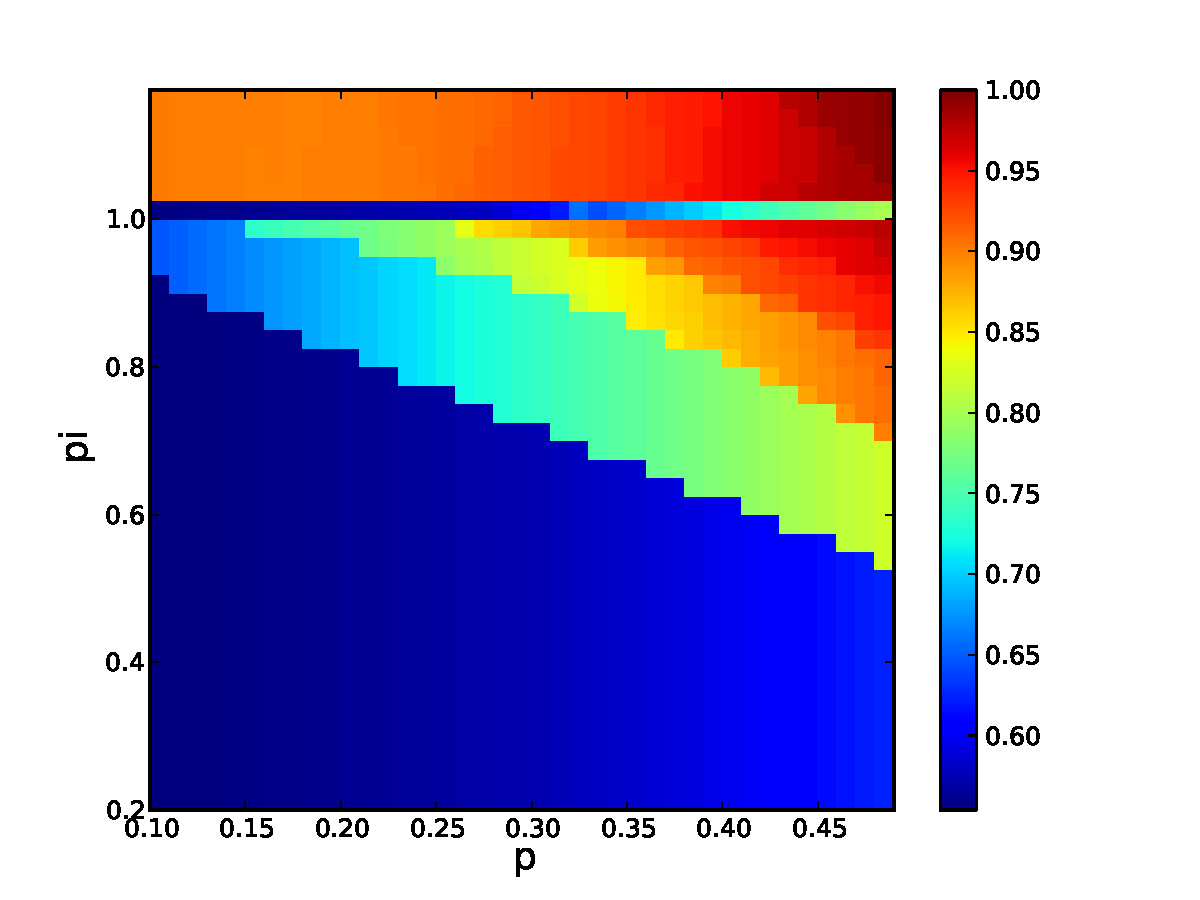
\includegraphics[width=\textwidth]{star_n10.pdf}
                \caption{Star}
        \end{subfigure}
        ~ 
        \begin{subfigure}[b]{0.3\textwidth}
                \centering
                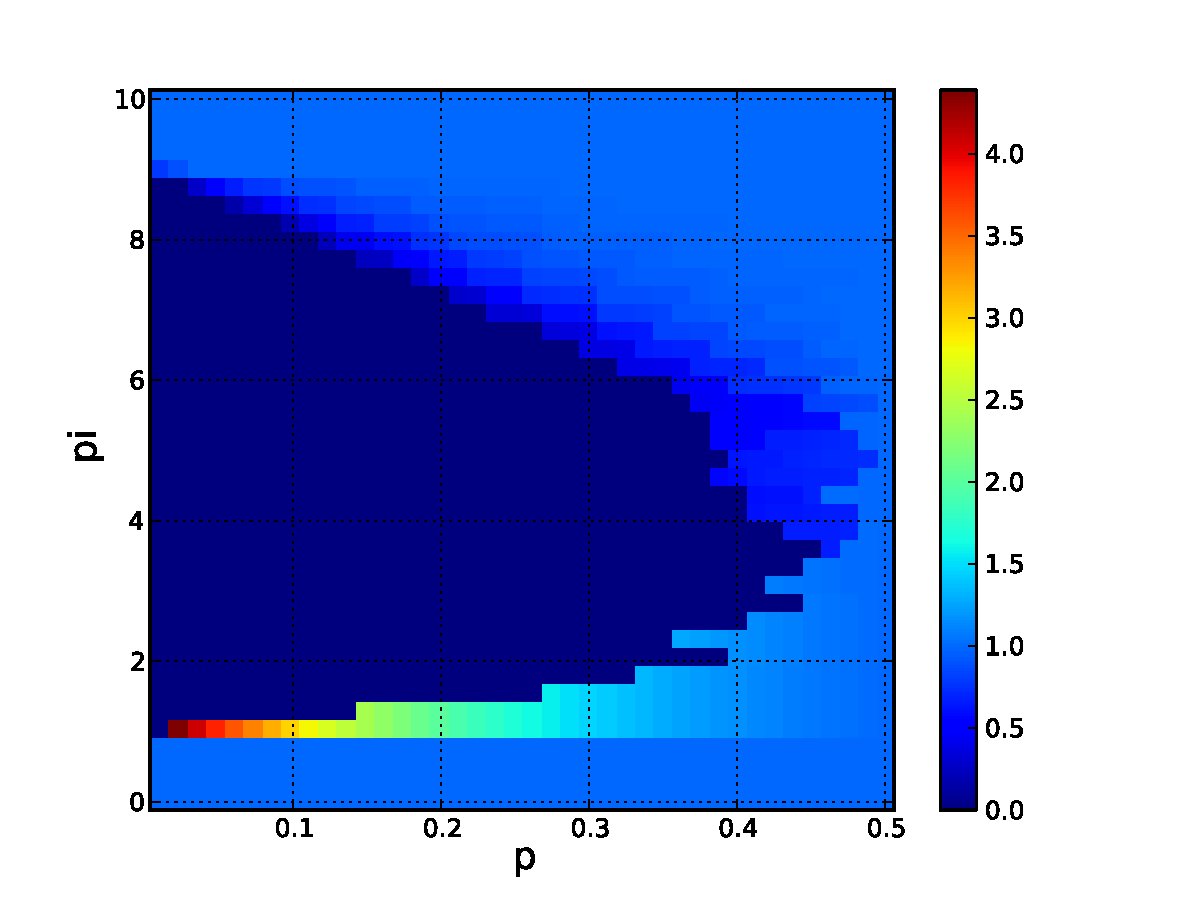
\includegraphics[width=\textwidth]{clique_n10.pdf}
                \caption{Clique}
        \end{subfigure}
        ~ 
        \begin{subfigure}[b]{0.3\textwidth}
                \centering
                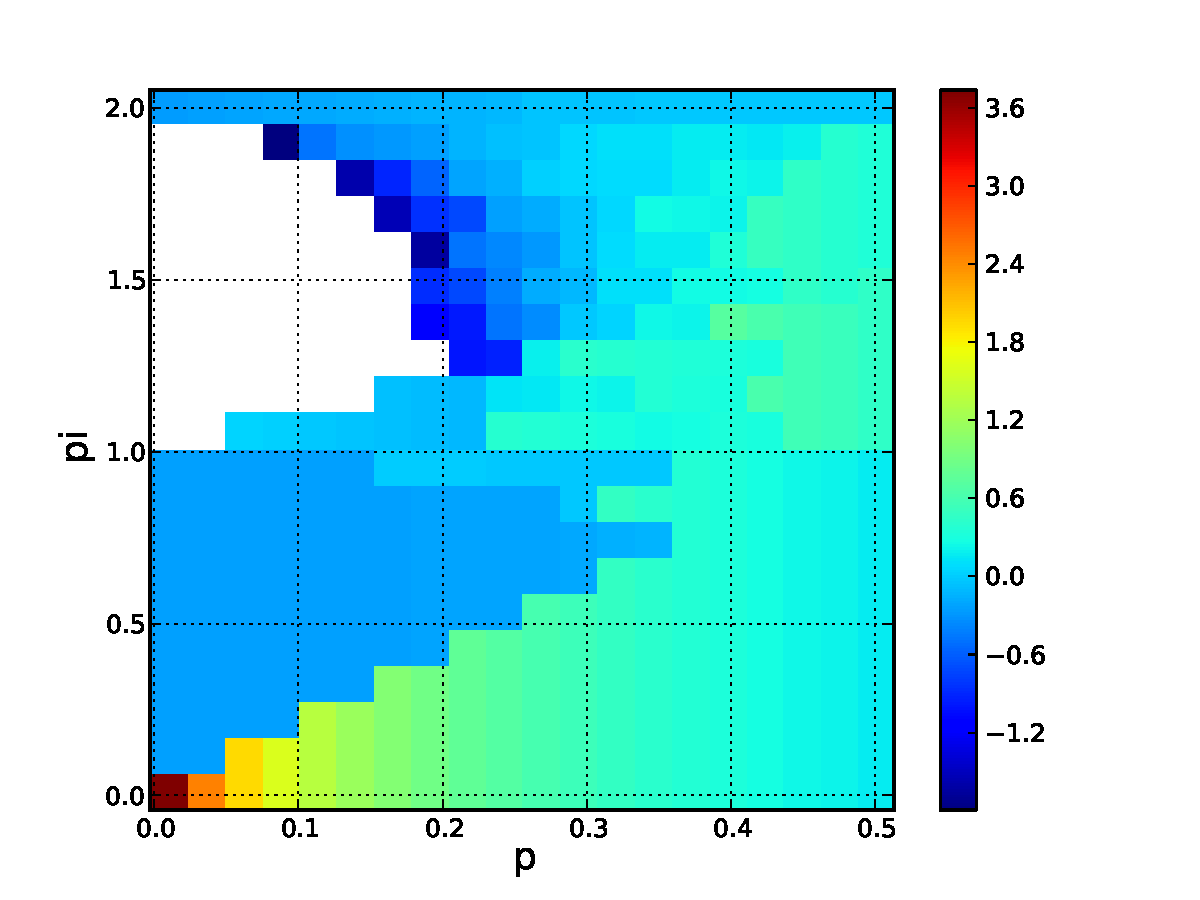
\includegraphics[width=\textwidth]{cloud_n10_r05_log.pdf}
                \caption{Cloud\footnotemark}
        \end{subfigure}
        \caption{Ratio of strategic:myopic Y adoptions for varying $p, \pi$.}
        \label{fig:ratio}
\end{figure}
\footnotetext{Log scale. White = $-\infty$ or $\log 0$}

\begin{figure}
        \centering
        \begin{subfigure}[b]{0.45\textwidth}
                \centering
                \includegraphics[width=\textwidth]{{p_ratio_pi0.9n20}.pdf}
                \caption{Varying p}
        \end{subfigure}
        ~ 
        \begin{subfigure}[b]{0.45\textwidth}
                \centering
                \includegraphics[width=\textwidth]{{pi_ratio_p0.45n20}.pdf}
                \caption{Varying pi}
        \end{subfigure}
        \caption{Ratio of strategic:myopic Y adoptions for varying $p, \pi$ on star graph.}
        \label{fig:ratio2}
\end{figure}

\begin{figure}
        \centering
        \begin{subfigure}[b]{0.45\textwidth}
                \centering
                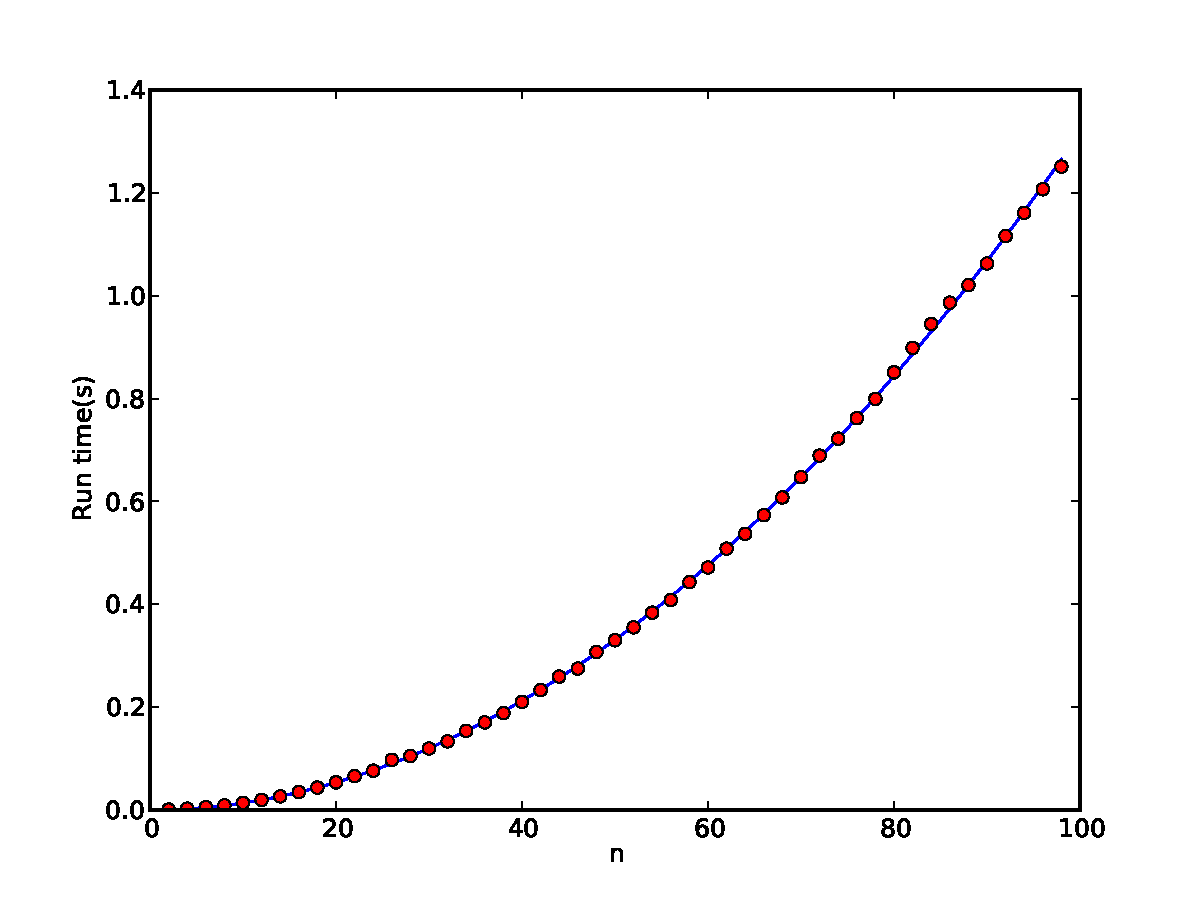
\includegraphics[width=\textwidth]{star_time.pdf}
                \caption{Star}
        \end{subfigure}
        ~ 
        \begin{subfigure}[b]{0.45\textwidth}
                \centering
                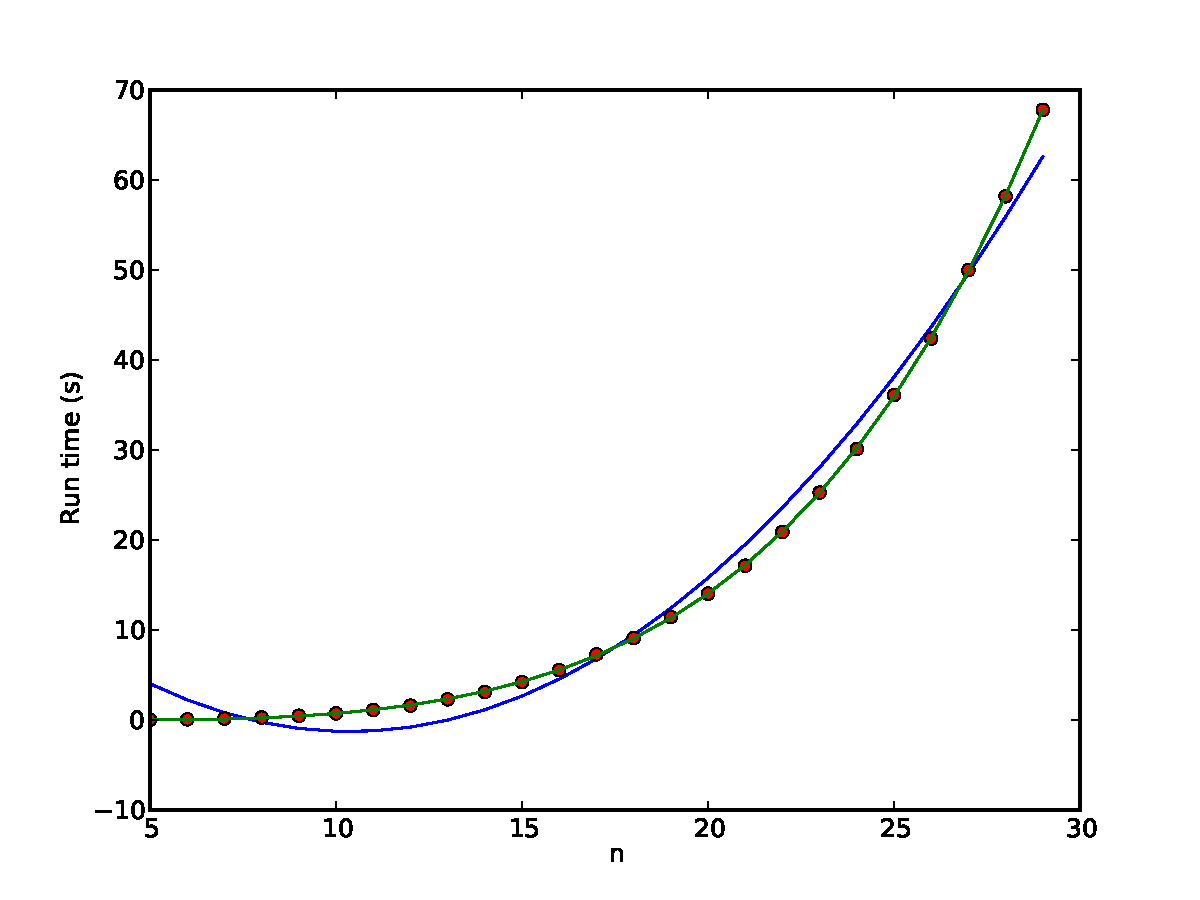
\includegraphics[width=\textwidth]{cloud_time.pdf}
                \caption{Cloud}
        \end{subfigure}
        \caption{Code runtime for varying graph size. Blue line is best quadratic fit, green line is best quartic fit.}
        \label{fig:time}
\end{figure}

\section{Future Work}

Our results are interesting and certainly show that the difference
between optimal play with myopic and strategic users is a complex
space even very simple block graphs. However, there are still a number
of interesting unexplored questions that we have not looked at in the
scope of the problem.

Despite the fact that obvious patterns don't exist in the performance
ratio, it is still possible that the performance ratio can be bounded
in certain circumstance beyond the star graph. Proving bounds on the
performance ratio could help characterize the discontinuous regions in
the plots where myopic superiority switches in favor of strategic
agents.

We have only shown a polynomial time algorithm for graphs where the
number of blocks is constant with respect to $n$. A further and
important step would be to come up with an algorithm for general
graphs, or to reduce the problem to another complexity class like PPAD
or NP.

The algorithm as it is presented only works for online
scheduling. This is a necessary condition to allow the dynamic
programming to work, however ongoing research may suggest that for
offline scheduling, myopic agents will always permit a higher number
of Yes nodes. Looking at performance bounds under offline scheduling
could pose an viable avenue to study performance difference where
online schedules became very complicated. It is not apparent how to
compute an optimal offline schedule efficiently for a block graph or
otherwise.

\bibliographystyle{plain}
\bibliography{references}

\end{document}
